\title{Computational Neurophysiology - Assignment 3}
\author{Ryan Spangler}
\date{\today}

\documentclass[12pt]{article}

\usepackage{commath}
\usepackage{graphicx}

\setcounter{secnumdepth}{0}

\begin{document}
\maketitle

\section{Potentiation}

Potentiation for a synapse is the adjustment in sensitivity to presynaptic activity by the incoming dendrites.  Potentiation is a complex process, but is clearly correlated with the presence of calcium in the postsynaptic cell.  Calcium is highly regulated in the cytoplasm, and can accumulate based on both presynaptic and postsynaptic activity.  Calcium is also buffered, so it takes a good deal of activity to saturate the buffers to the degree that calcium actually concentrates.  

The presence of higher concentrations of calcium lead to long-term potentiation, whereas lower concentrations induce long-term depression.  If the incoming stimulus is high-frequency, the concentration of postsynaptic calcium will rise and subsequently cause long-term potentiation, and conversely the lower frequency stimuli will lead to long-term depression.

\section{Plasticity}

Using a simulation of the BCM model for synaptic plasticity I was able to explore the dynamics under a variety of conditions.  This simulation uses a simplified model with 1000 synapses with randomly distributed weights and presynaptic activity given by a poisson process.  Postsynaptic activity is modeled as an instantaneous product of the presynaptic weights and activity:

$$ v=\mathbf{w}\cdot\mathbf{u} $$

while the change in weights is given by the postsynaptic and presynaptic activity relative to the threshhold:

$$ \tau_w\od{\mathbf{w}}{t}=v\mathbf{u}(v-\theta) $$

The threshhold $\theta$ itself can be either static, so that $\od{\theta}{t}=0$, or use a sliding value based on the postsynaptic activity itself:

$$ \tau_\theta\od{\theta}{t}=v^2-\theta $$

Both the weights vector and the threshhold have corresponding time constants $\tau$ which govern how quickly each value changes.  

Without the ability to shift the threshhold to compensate for the postsynaptic activity the BCM rule is unstable, and must use saturation values to keep growth in check.  In the trials I ran, setting $\tau_\theta=1$ and $\tau_w=100$, if the activity never gets above the threshhold the system quickly tends to zero:

\vspace{15pt}
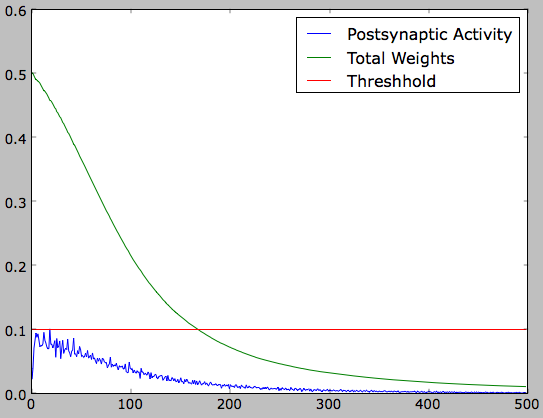
\includegraphics[scale=0.5]{static.png}
\vspace{15pt}

On the other hand, if activity ever did rise above the threshhold, the weights inevitably all reached saturation and stayed there, destroying any variability in the impact of any single presynaptic activity.  Here is the same system with a saturation of 1 and the weights initially high enough to encourage activity:

\vspace{15pt}
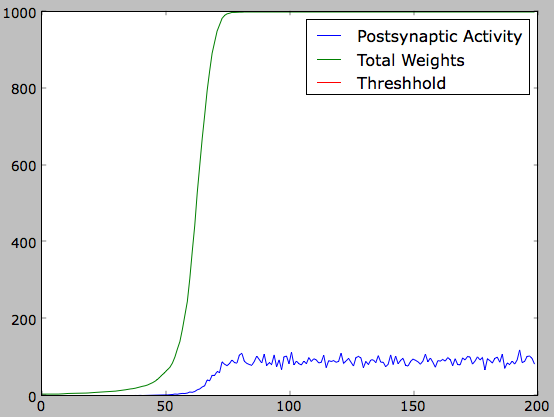
\includegraphics[scale=0.5]{staticgrowth.png}
\vspace{15pt}

The sum of all weights zooms to 1000 and stays there, and since there are 1000 synapses this means that all weights are at saturation.

If the threshhold $\theta$ is allowed to slide in response to activity however, the BCM rule stabilizes and activity revolves around a fixed point:

\vspace{15pt}
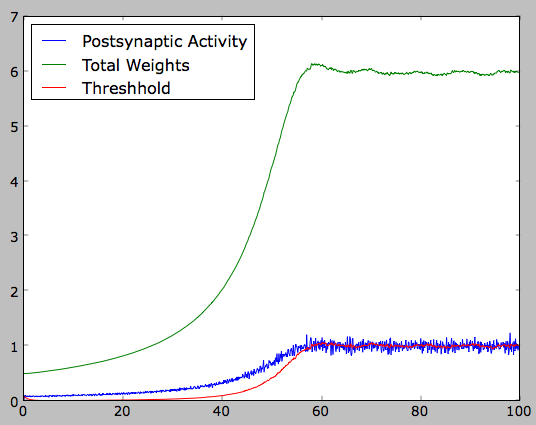
\includegraphics[scale=0.5]{sliding.png}
\vspace{15pt}

In this diagram the weights behave in a similar way to the fixed threshhold saturation system of before, but the total finds its own balance with the activity of the postsynaptic cell, rather than maxxing out at the saturation point for every weight.  If the firing rate is halved, similar dynamics play out over a longer timescale, and at a higher total weight value:

\vspace{15pt}
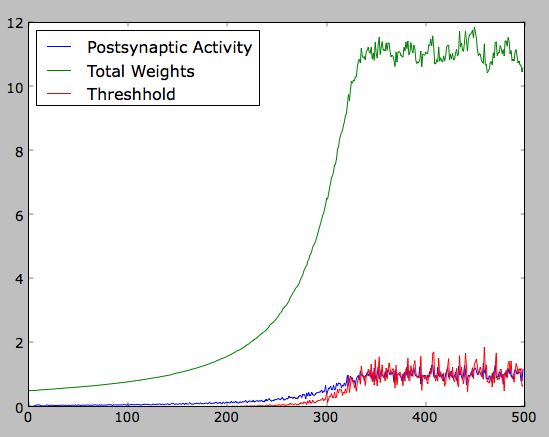
\includegraphics[scale=0.6]{halfrate.png}
\vspace{15pt}

For this trial, the rate was halved, which means about half as much activity is coming into the cell.  The threshhold compensated for the drop in activity by emerging with about twice the total weight strength.  Also, while the earlier trial balanced out about 60 time steps into the simulation, at half rate it took close to 350 time steps to reach the fixed point, or almost six times as long.  Also, the activity is more chaotic, with a wider variability, in the trial with the slower rate.

Interpreting the results in biophysical terms, if the BCM is a plausible model for synaptic plasticity then there must be some biophysical corrolary to the sliding threshhold dynamics based on postsynaptic activity.  One possibility is that since calcium concentration is directly dependent on postsynaptic activity, a mechanism based on the presence or absence of calcium could emulate the sliding threshhold used in this model to ensure overall stability of the weight strengths.  Under high activity the calcium concentration would rise, requiring a higher activity to raise weight strengths and increasing the likelihood that weights would decrease, no matter what the postsynaptic activity was.

\end{document} 
